% Springer LNCS conference-format submission draft.
\documentclass[runningheads,a4paper]{llncs}

\usepackage[T1]{fontenc}
\usepackage[utf8]{inputenc}
\usepackage{graphicx}
\usepackage{booktabs}
\usepackage{amsmath,amssymb}
\usepackage{url}
\usepackage{microtype}

\graphicspath{{figures/}{figures/v2/}{tikz/}}

\newcommand{\tinker}{\textsc{Tinker}}
\newcommand{\grpo}{\textsc{GRPO}}
\newcommand{\zvf}{\textsc{ZVF}}
\newcommand{\gu}{\textsc{GU}}
\newcommand{\ours}{\textsc{TinkerRL Audit}}

\begin{document}

\title{Reward Contrast, Not Algorithm Labels:\\
A Diagnostic Audit of Group-Relative Reinforcement Learning for LLMs}
\titlerunning{Reward Contrast, Not Algorithm Labels}

\author{Arvind C R\inst{1} \and
Sandhya Jeyaraj\inst{1} \and
Madhu Kumara L\inst{1} \and
Mohammad Rafi\inst{1} \and
Dhruva N Murthy\inst{1} \and
Arumugam K\inst{1} \and
Anwesh Reddy Paduri\inst{2} \and
Narayana Darapaneni\inst{3}}
\authorrunning{A. C R et al.}

\institute{PES University, Bengaluru, India\\
\email{arvindcr4@gmail.com}
\and
Great Learning / PES University, India\\
\email{anwesh@greatlearning.in}
\and
Northwestern University / Great Learning, USA\\
\email{narayana.darapaneni@northwestern.edu}}

\maketitle

\begin{abstract}
Group-relative reinforcement learning has become a common recipe for post-training large language models, but the algorithm name alone rarely specifies the full experimental treatment. This paper presents a diagnostic audit of a critic-free, group-relative training runner inspired by GRPO. The goal is not to claim a new optimizer or a leaderboard result, but to determine when a particular model--reward--sampler--stack combination has usable reward contrast. We formalize the mixed-group probability that a prompt produces both successful and unsuccessful completions in a group, and operationalize it through Zero-Variance Fraction (ZVF) and Gradient Utilization (GU). Across 22 validation runs, a first-five-step rule using high ZVF and low reward catches the observed collapsed runs, but the result is power-limited and should be read as triage rather than prediction. On GSM8K, the clean paired held-out result for Qwen3-8B improves only from 82.0\% to 83.3\% and is not statistically significant ($p=0.26$). We also observe large stack effects: under a nominally matched visible GRPO configuration, the Tinker-managed runner reaches 84.4\% last-10 training reward, while a TRL/Modal run reaches 5.0\%. These findings support a conservative conclusion: online reward curves are evidence about training dynamics, not capability, and PPO/GRPO/DPO labels must be accompanied by full-stack reporting.

\keywords{Group-relative reinforcement learning \and GRPO \and Large language models \and Reward contrast \and GSM8K \and Reproducibility}
\end{abstract}

\section{Introduction}
\label{sec:introduction}

Reinforcement learning for language-model post-training is often described
through compact algorithm labels: PPO, DPO, GRPO, or a recent variant thereof.
Those labels are useful, but they are incomplete. In practice, an LLM
post-training result depends on the base model, instruction tuning, reward
parser, rollout sampler, loss mask, reference-policy treatment, LoRA
configuration, backend, checkpoint-selection rule, and evaluation harness.
This echoes the reproducibility problem identified in earlier deep-RL work:
without a complete experimental treatment, algorithm comparisons are unstable
and difficult to interpret~\cite{henderson2018deep,agarwal2021deep}.

This paper studies a group-relative RL runner inspired by GRPO, rather than a
canonical DeepSeekMath GRPO implementation~\cite{shao2024deepseekmath}. The
runner preserves the critic-free group-relative reward-contrast mechanism, but
the implementation differs from canonical PPO-style policy optimization: it
does not retain all ratio clipping and reference-policy details, and some
experiments use proxies such as schema compliance or short-horizon verifier
rewards. We therefore avoid claims that the runner represents GRPO as an
algorithmic family. The central question is narrower: when does the sampled
group contain enough reward diversity to provide a usable learning signal?

For binary or verifier-like rewards, a prompt that always receives all-correct
or all-incorrect completions contributes little or no group-relative gradient.
If the current policy succeeds on prompt $x$ with probability $p_x$ and group
size $G$, the probability of a mixed, gradient-carrying group is approximated by
\begin{equation}
P(\mathrm{usable}) \approx
\frac{1}{N}\sum_x \left[1-(1-p_x)^G-p_x^G\right].
\label{eq:mixed_group}
\end{equation}
This expression is the paper's organizing mechanism. It clarifies why
warm-starts, reward density, group size, and task difficulty can matter more
than the method name. A very weak policy collapses into all-failure groups; a
near-saturated policy collapses into all-success groups; both cases reduce the
useful contrast that a group-relative update can exploit.

We operationalize this mechanism using Zero-Variance Fraction (\zvf) and
Gradient Utilization (\gu). \zvf{} is the fraction of prompts whose sampled
group receives identical rewards; \gu{} is $1-\zvf$. High \zvf{} with low reward
indicates cold-start collapse, high \zvf{} with high reward indicates
saturation, and low \zvf{} indicates within-group contrast. These are diagnostic
statistics, not final capability metrics. The distinction is central because
training rewards are generated inside the training environment and can reflect
parser artifacts, prompt difficulty, format learning, or checkpoint selection.

Table~\ref{tab:claim_evidence} summarizes the evidence hierarchy used
throughout the paper. We treat online training reward as dynamics evidence,
held-out GSM8K accuracy as limited capability evidence, and tool-use/schema
scores as telemetry unless execution success is independently evaluated.

\begin{table}[t]
\centering
\caption{Claim--evidence hierarchy used in this Springer-format submission.}
\label{tab:claim_evidence}
\small
\begin{tabular}{p{0.29\linewidth}p{0.39\linewidth}p{0.22\linewidth}}
\toprule
\textbf{Claim} & \textbf{Evidence used} & \textbf{Interpretation} \\
\midrule
Reward contrast is required & Mixed-group probability and ZVF/GU telemetry & Mechanistic diagnostic \\
ZVF/GU help early triage & First-five-step collapse rule on 22 runs & Triage, not prediction \\
Training reward is not capability & Qwen3-8B held-out GSM8K $82.0\%\to83.3\%$ & Narrow null result \\
Algorithm labels are incomplete & Tinker-vs-TRL stack gap under nominal config & Reporting warning \\
\bottomrule
\end{tabular}
\end{table}

The contributions are fourfold. First, we express the group-relative signal
bottleneck through the mixed-group probability in Eq.~\ref{eq:mixed_group}.
Second, we use \zvf{} and \gu{} as lightweight triage diagnostics for collapse,
saturation, and usable contrast. Third, we show that the clean held-out GSM8K
effect is small and not statistically significant, despite strong online reward
traces in selected runs. Fourth, we show that nominally similar GRPO
configurations can diverge sharply across stacks, motivating more complete
reporting in LLM RL studies.

\section{Literature Review}
\label{sec:literature}

\subsection{Policy optimization and preference learning for LLMs}

PPO remains the dominant policy-gradient method behind RLHF-style training
pipelines~\cite{schulman2017proximal,ouyang2022training}. Early RLHF systems
used learned reward models built from human preference data, then optimized
policy behavior against those reward models~\cite{christiano2017deeprlhf,stiennon2020summarize,bai2022hhrlhf}. The success of these systems made PPO a
default baseline for instruction following, summarization, and assistant
alignment. However, PPO results are sensitive to KL control, value estimation,
sampling, reward scaling, and implementation details. These issues become more
pronounced in language-model settings, where tokens, completions, prompts, and
sequence-level rewards interact.

DPO reframed preference optimization as a supervised contrastive objective,
removing explicit rollouts and learned value functions from the training
loop~\cite{rafailov2024direct}. DPO and related preference losses provide a
useful foil for online RL because they trade environment interaction for
offline preference data. For this paper, their importance is conceptual:
several group-relative updates can be interpreted as contrastive procedures
over sampled completions. A prompt contributes signal only when the sampled
responses differ in reward or preference status.

GRPO gained prominence through DeepSeekMath and subsequent reasoning models,
which used groups of completions and group-relative advantages to reduce the
need for a learned critic~\cite{shao2024deepseekmath,guo2025deepseekr1}. In
the canonical formulation, GRPO is still embedded in a full training recipe:
base model, reward source, sampling temperature, group size, reference
regularization, length handling, and loss masking all matter. Recent open
model reports such as Qwen3 further show that the model family and training
lineage shape the apparent effect of post-training~\cite{qwen2025qwen3}. The
literature therefore supports the premise that ``GRPO'' is not a sufficient
experimental description.

\subsection{Reasoning rewards and verifier-based training}

Mathematical reasoning has become a common setting for verifier-based RL
because many answers can be checked with exact or near-exact parsers.
GSM8K-style word problems provide a useful but narrow benchmark for this
purpose~\cite{cobbe2021training}. Process reward models extend this idea from
final-answer checking to step-level supervision. Work such as Let's Verify
Step by Step, Math-Shepherd, and PRM800K shows that intermediate reasoning
signals can be valuable for mathematical problem solving~\cite{lightman2024stepbystep,wang2024mathshepherd,uesato2022prm800k}. These papers motivate richer reward
signals, but they also highlight a risk: once the reward is only a proxy for
the intended capability, the reward curve must not be read as capability
itself.

Reward-model and automatic-evaluator studies reinforce this caution.
RewardBench and length-controlled evaluation work show that reward and
evaluation artifacts can change conclusions if length, format, or parser
behavior is not controlled~\cite{lambert2024rewardbench,dubois2024lengthcontrolled}.
Reward hacking is not a remote theoretical concern; it is a recurring failure
mode when an optimizer exploits the measurement channel rather than the target
behavior~\cite{skalse2022specificationgaming}. In group-relative RL, a related
failure arises when the reward environment is too sparse or too easy. Sparse
failure produces all-zero groups; saturation produces all-one groups; both
states can hide the absence of useful contrast.

\subsection{Frameworks and reproducibility}

The current RLHF ecosystem includes TRL, OpenRLHF, veRL/HybridFlow, Tinker, and
other stack-specific implementations~\cite{vonwerra2022trl,hu2024openrlhf,sheng2024verl,thinkingmachines2024tinker}. These systems differ in rollout
scheduling, accelerator usage, optimizer behavior, tokenizer handling,
completion masking, logging, checkpointing, and failure recovery. A visible
hyperparameter table is therefore necessary but insufficient. Two runs may
share model, group size, learning rate, seed, and dataset while differing in
backend semantics or parser behavior.

This reproducibility problem is continuous with prior deep-RL findings.
Henderson et al. showed that performance can vary with random seeds and
implementation choices, while Agarwal et al. argued for aggregate metrics and
uncertainty-aware reporting~\cite{henderson2018deep,agarwal2021deep}. We apply
the same ethos to LLM RL: report evidence levels, separate dynamics from
capability, and avoid single-number algorithm rankings when stacks differ.
For multiple comparisons we use the Benjamini--Hochberg false-discovery-rate
procedure where appropriate~\cite{benjamini1995controlling}.

\subsection{Zero-variance and difficulty filtering}

The most directly related recent work studies how to recover signal from
zero-variance or poorly selected prompts. RL-ZVP proposes advantage shaping to
use prompts that would otherwise have zero reward variance, while online
difficulty filtering selects prompts with intermediate success probability so
that sampled groups retain contrast~\cite{rlzvp2025,bae2025online}. Our work is
complementary. We do not propose a new optimizer or curriculum. Instead, we
measure whether a given stack currently has useful signal and how much
evidential weight its reward trajectory deserves.

\section{Model Details and Data}
\label{sec:model_data}

\subsection{Training stack and model families}

The audit corpus uses a critic-free, group-relative training runner built
around the Tinker API for managed forward/backward, sampling, optimization, and
checkpointing. The primary experiments use Qwen-family models because they
provide a dense scale ladder and strong public reasoning baselines. Additional
runs use Llama, DeepSeek, Nemotron, and MoE variants as auxiliary probes. The
most important controlled result is the Qwen3-8B GSM8K held-out comparison,
which uses five seeds and a separated evaluation slice.

The runner is intentionally described as GRPO-style rather than canonical GRPO.
Its shared feature is the use of multiple completions per prompt and
group-relative reward normalization. The stack does not support all canonical
GRPO implementation details in every run, and the paper does not claim that
omitting those details is algorithmically harmless. This is why all results are
framed as stack-conditioned evidence.

\subsection{Datasets, rewards, and splits}

The main reward environment is GSM8K-style mathematical reasoning. During
training, answers are parsed through a boxed-answer verifier and converted to a
binary correctness reward. Held-out evaluation is reported separately and is
never pooled with online reward. Auxiliary environments include arithmetic
sanity tasks, HumanEval-style code probes, and tool-call schema compliance
tasks. These auxiliary rows are included to study reward contrast and stack
behavior, not to claim broad agentic capability.

Table~\ref{tab:data_protocol} summarizes the data and measurement roles. The
important distinction is that training reward, held-out accuracy, and proxy
schema scores answer different questions.

\begin{table}[t]
\centering
\caption{Data and measurement protocol.}
\label{tab:data_protocol}
\small
\begin{tabular}{p{0.24\linewidth}p{0.30\linewidth}p{0.34\linewidth}}
\toprule
\textbf{Setting} & \textbf{Reward or metric} & \textbf{Permitted interpretation} \\
\midrule
GSM8K training & Binary boxed-answer reward & Online dynamics and reward contrast \\
GSM8K held-out & Greedy boxed-answer accuracy & Narrow capability/generalization check \\
Arithmetic sanity & Exact answer accuracy & Stack sanity and parser validation \\
Tool-call probe & JSON/schema compliance & Format telemetry, not execution success \\
Code probe & Custom sandbox score & Auxiliary reward-environment evidence \\
\bottomrule
\end{tabular}
\end{table}

\subsection{Diagnostics and statistical checks}

For each group-relative run, we compute \zvf{} and \gu{} when per-prompt group
rewards are available. A prompt has zero reward variance if all $G$ completions
receive the same binary reward. The first-five-step collapse rule flags a run
when early \zvf{} is at least $80\%$ and early reward is at most $5\%$.
This rule is deliberately simple so that it can be used during training rather
than after a full analysis pass.

For held-out GSM8K we report accuracy, paired comparisons, and $p$-values
instead of relying on online reward. Because the clean held-out comparison is
small and not significant, it acts as a constraint on the paper's claims.
When tables combine single-seed traces, interrupted runs, or proxy rewards, we
label them as exploratory and do not treat them as causal algorithm
comparisons.

\section{Results}
\label{sec:results}

\subsection{Held-out GSM8K capability}

The cleanest capability check is the Qwen3-8B held-out GSM8K comparison.
Across five seeds and 200 held-out prompts, the base model obtains 82.0\%
accuracy and the post-training checkpoint obtains 83.3\%. The gain is small
and not statistically significant ($p=0.26$). This result is the main
constraint on interpretation: online reward improvements should not be
promoted to broad reasoning claims.

\begin{table}[t]
\centering
\caption{Core quantitative results. Online reward rows are dynamics evidence;
the held-out row is the narrow capability check.}
\label{tab:core_results}
\small
\begin{tabular}{p{0.25\linewidth}p{0.16\linewidth}p{0.17\linewidth}p{0.28\linewidth}}
\toprule
\textbf{Experiment} & \textbf{Metric} & \textbf{Value} & \textbf{Interpretation} \\
\midrule
Qwen3-8B base vs. post-train & Held-out GSM8K & $82.0\%\to83.3\%$, $p=0.26$ & Small, non-significant lift \\
Top-10 selected checkpoints & Held-out GSM8K & $87.2$--$95.0\%$ & Checkpoint-selection audit \\
Llama-3.3-70B, four seeds & Held-out GSM8K & all $95.0\%$ & Last-10 variance is mostly sampling noise \\
Tinker Qwen3-8B, $G=8$ & Last-10 train reward & $84.4\%$ & Strong online reward under this stack \\
TRL/Modal Qwen3-8B, $G=8$ & Last-10 train reward & $5.0\%$ & Stack sensitivity under nominal config \\
\bottomrule
\end{tabular}
\end{table}

\subsection{Stack sensitivity}

Under a nominally matched visible GRPO configuration (Qwen3-8B, group size
$G=8$, learning rate $10^{-5}$, GSM8K-500, 30 steps, seed 42), the
Tinker-managed runner reaches 84.4\% last-10 training reward while the
TRL/Modal run reaches 5.0\%. This 17$\times$ gap is not evidence that one
framework is universally better. It is evidence that model, sampler, reward
parser, backend, loss mask, optimizer, and logging semantics are part of the
treatment.

\begin{figure}[t]
\centering

\includegraphics[width=0.78\linewidth]{framework_comparison.pdf}
\caption{Stack-sensitivity probe under nominally matched visible GRPO
configuration. The figure supports a reporting warning, not a framework
leaderboard.}
\label{fig:framework_gap}
\end{figure}

\subsection{Group size and usable reward contrast}

The mixed-group mechanism predicts that group size changes signal availability
nonlinearly. Very small groups may fail to sample successes; very large groups
increase rollout cost and can still saturate on easy prompts. In the Qwen3-8B
GSM8K ablation, $G=8$ gives the strongest last-10 training reward among the
reported settings, while $G=16$ degrades.

\begin{table}[t]
\centering
\caption{Qwen3-8B GSM8K group-size ablation. Values are online training reward,
not held-out accuracy.}
\label{tab:group_size}
\small
\begin{tabular}{cccc}
\toprule
\textbf{Group size} & \textbf{Steps} & \textbf{Peak reward} & \textbf{Last-10 reward} \\
\midrule
$G=2$  & 30 & 50.0\%  & 37.5\% \\
$G=4$  & 30 & 75.0\%  & 52.1\% \\
$G=8$  & 30 & 100.0\% & 84.4\% \\
$G=16$ & 30 & 71.9\%  & 38.0\% \\
\bottomrule
\end{tabular}
\end{table}

\begin{figure}[t]
\centering
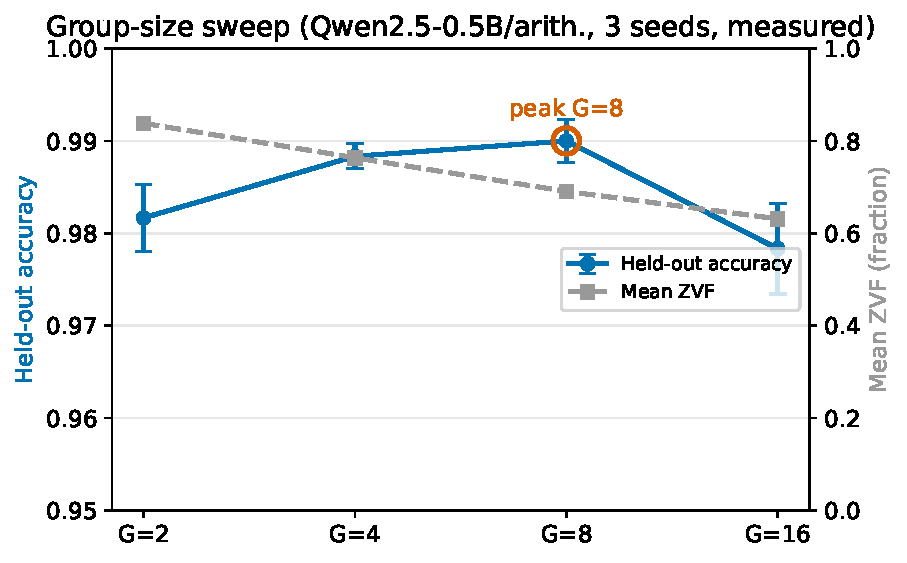
\includegraphics[width=0.76\linewidth]{group_size_ablation.pdf}
\caption{Empirical group-size ablation on Qwen3-8B/GSM8K. The strongest
training reward occurs at $G=8$, consistent with the need for mixed-reward
groups rather than only larger rollout batches.}
\label{fig:group_size}
\end{figure}

\subsection{ZVF and early triage}

Across the de-duplicated validation set, the fixed rule
\zvf{}$\geq80\%$ and reward $\leq5\%$ within the first five steps catches the
two observed collapsed runs and produces no false positives. Because there are
only two positive collapse cases, this should not be presented as a calibrated
predictor. Its practical use is triage: when early rewards and \zvf{} indicate
cold-start collapse, the operator can stop the run, warm-start the model,
densify the reward, adjust task difficulty, or change group size.

\section{Discussion and Conclusion}
\label{sec:discussion}

\subsection{What the results mean}

The audit supports a conservative view of group-relative RL. The useful signal
is not created by the acronym; it is created when the current policy, reward
function, sampler, and task distribution produce mixed-reward groups. This is
why \zvf{} and \gu{} are useful. They expose a simple failure mode that can
otherwise be hidden behind noisy reward curves: the run may be updating on too
few informative groups, or it may be saturated before any meaningful
generalization has been demonstrated.

The most important negative result is the held-out GSM8K control. A training
run can produce strong online reward while the clean held-out comparison shows
only an 82.0\% to 83.3\% increase with $p=0.26$. Therefore, training reward is
evidence about the reward environment and optimization dynamics. It is not, by
itself, evidence of improved reasoning capability. The same logic applies more
strongly to tool-call schema rewards and custom code sandboxes: those probes
are useful for detecting whether the stack can optimize a signal, but they do
not establish end-to-end agentic competence.

\subsection{Limitations}

The study has several limits. Many runs are short-horizon and single-seed.
Some large-model traces are interrupted and are reported only as partial
training-reward evidence. The runner is GRPO-style rather than canonical GRPO,
so its results should not be generalized to every GRPO implementation. The
HumanEval-style and tool-use probes use custom scoring environments, and their
numbers should not be compared to public benchmark leaderboards. Finally, the
ZVF triage rule is validated on a small number of collapse cases and should be
treated as an operational heuristic until tested on a larger corpus.

\subsection{Conclusion}

This paper reformats the TinkerRL audit as a Springer conference submission and
states the central result plainly: reward contrast, not algorithm labels,
determines whether a group-relative LLM RL run has usable signal. The
mixed-group probability explains the mechanism, \zvf{}/\gu{} expose the
operational state of a run, and the held-out GSM8K result constrains the
capability claim. The practical recommendation is to report the full stack,
separate online reward from held-out evaluation, and use early contrast
diagnostics before interpreting PPO, GRPO, or DPO outcomes as algorithmic
evidence.

\bibliographystyle{splncs04}
\bibliography{springer_refs}

\end{document}
